%----------------Cap_02----------------%
\chapter{Detalhamento do Projeto}

Este capítulo apresenta o detalhamento completo da fase experimental do projeto, cobrindo a descrição do sistema físico, a modelagem e identificação do modelo dinâmico e a implementação do controlador no hardware embarcado. A arquitetura da solução, evidenciando as fases de desenvolvimento offline e a operação de controle em tempo real, está sintetizada na visão geral do diagrama de blocos da Figura~\ref{fig:diagrama-blocos-projeto}. As seções subsequentes detalham o funcionamento de cada módulo ilustrado, partindo da instrumentação e caracterização da planta até a validação do algoritmo de controle no microcontrolador.

\begin{figure}[h]
    \centering
    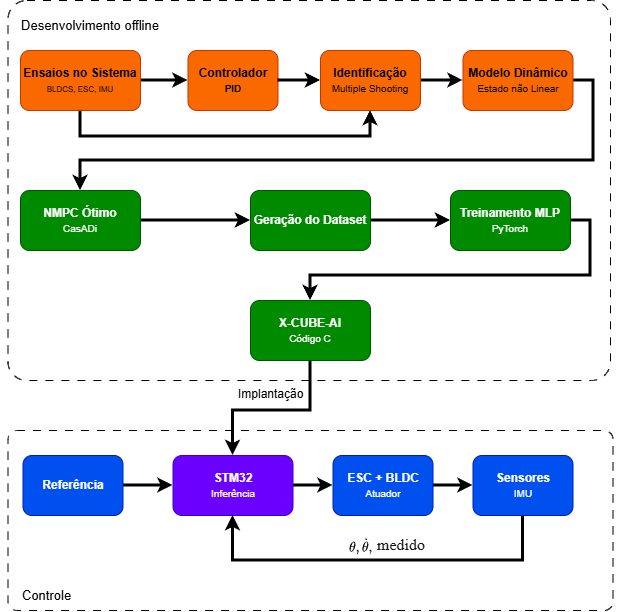
\includegraphics[width=1\textwidth]{img/blocos-projeto.png}
    \caption{Diagrama de Blocos do Projeto}
    \label{fig:diagrama-blocos-projeto}
\end{figure}


% ------------------------------------------------------------
\section{Descrição do Sistema Físico}
A infraestrutura física e mecânica da bancada do aeropêndulo utilizada neste trabalho foi originalmente projetada e construída por \citeonline{lima2025}. O sistema mecânico pré-existente e reaproveitado compreende a base de madeira, as torres de suporte, o eixo de alumínio instrumentado e a haste pendular contendo o motor \textit{brushless} (BLDC) acoplado. 

O aeropêndulo atua como um sistema de um grau de liberdade, composto por esse braço rígido livre para rotacionar em torno do eixo horizontal fixo. A posição angular $\theta$ é medida em relação à horizontal, sendo $0^\circ$ definido quando o sistema está em repouso com o motor na posição inferior.

% ------------------------------------------------------------
\subsection{Estrutura Mecânica}

A estrutura física do aeropêndulo é montada sobre uma base de madeira compensada. Dois suportes triangulares confeccionados em MDF sustentam  o eixo de rotação do sistema. As faces foram unidas por colagem  nas arestas, e peças impressas em 3D foram fixadas nos cantos de cada torre e  parafusadas à base.

Para fixar o eixo de alumínio às torres, é utilizado um cuboide retangular contendo  um rolamento de esferas, permitindo que o eixo gire livremente. No centro do eixo foi usinado e rosqueado um furo para encaixe da haste  do pêndulo.

A haste rosqueada também permite a fixação e remoção facilitada de contrapesos, que foram usinados e rosqueados para se encaixar diretamente na haste. Um suporte impresso em 3D acopla o motor BLDC à extremidade da haste. A propulsão é gerada por uma hélice bipá de passo fixo. Um alojamento impresso em 3D para a Unidade de Medição Inercial (IMU) foi desenvolvido e fixado ao eixo de rotação, responsável por capturar o angulo do sistema. A Figura~\ref{fig:montagem-bancada} ilustra o formato atual da bancada. Os principais parâmetros construtivos do sistema são resumidos na Tabela~\ref{tab:componentes_mecanicos}.

\begin{figure}[h]
    \centering
    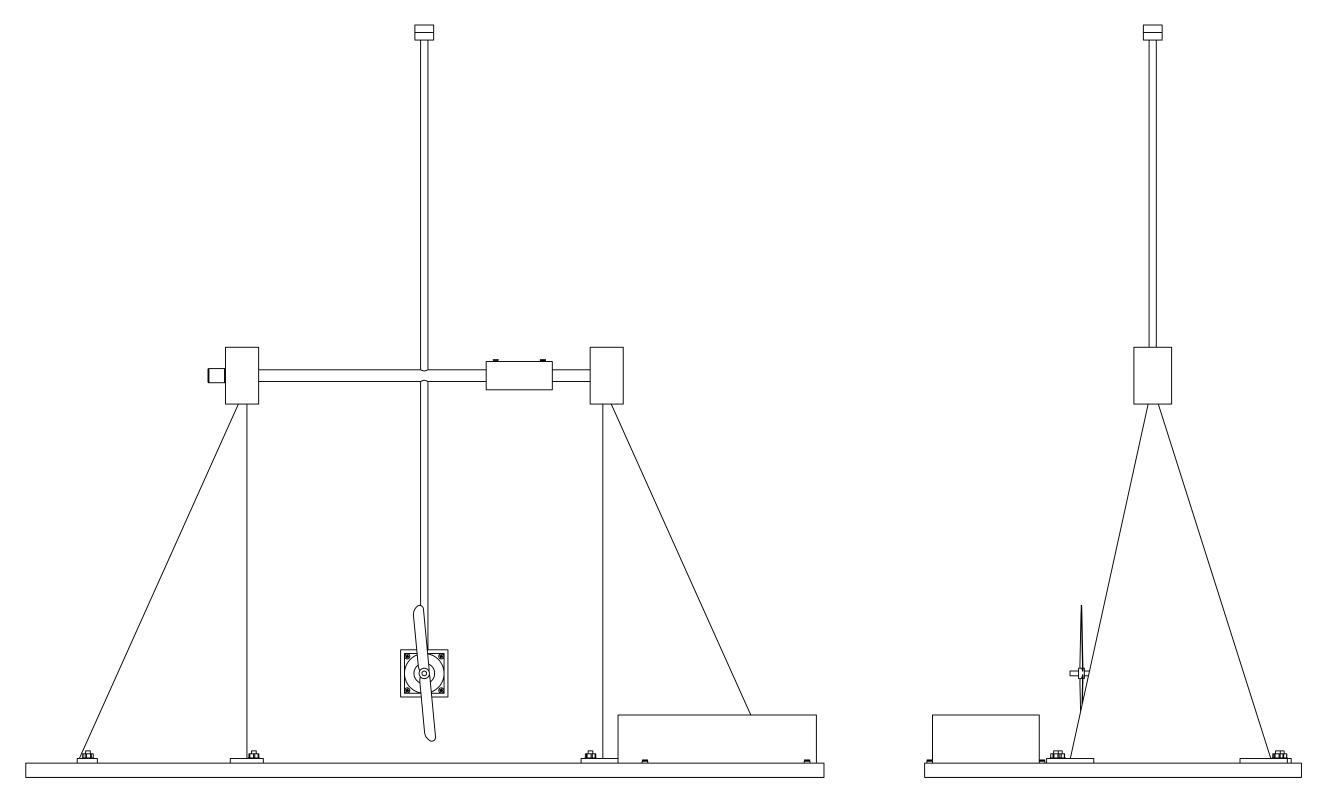
\includegraphics[width=1\textwidth]{img/montagem-bancada.png}
    \caption{Desenho da Bancada}
    \label{fig:montagem-bancada}
\end{figure}



\begin{table}[h!]
    \centering
    \caption{Componentes mecânicos do aeropêndulo}
    \label{tab:componentes_mecanicos}
    \begin{tabular}{ll}
        \hline
        \textbf{Componente}       & \textbf{Material / Modelo}              \\
        \hline
        Base                      & Madeira compensada                      \\
        Torres de suporte         & MDF com reforços em PLA (impressão 3D)  \\
        Eixo de rotação           & Alumínio                                \\
        Mancal                    & Rolamento de esferas                    \\
        Haste do pêndulo          & Haste rosqueada                         \\
        Contrapesos               & Peças rosqueadas (ajustáveis)           \\
        Suporte do motor          & PLA (impressão 3D)                      \\
        Alojamento da IMU         & PLA (impressão 3D)                      \\
        Motor                     & A definir                           \\
        Hélice                    & Bipá, passo fixo                     \\
        \hline
    \end{tabular}
\end{table}

% ------------------------------------------------------------
\subsection{Sensores}

% ------------------------------------------------------------
\subsubsection{Unidade de Medição Inercial (IMU)}

A unidade de medição inercial utilizada é o ICM-20948, fabricado pela InvenSense (TDK), um dispositivo MEMS de 9 eixos que integra giroscópio triaxial, acelerômetro triaxial e magnetômetro triaxial em um único encapsulamento QFN de 3$\times$3$\times$1\,mm \cite{invensense2021icm20948}.

A comunicação com o microcontrolador é realizada via I$^2$C no modo \textit{fast} (400\,kHz), utilizando os pinos SCL e SDA do STM32. O endereço I$^2$C do dispositivo é definido pelo nível lógico do pino AD0, com AD0 em nível baixo, o endereço é \texttt{0x68}. Os dados do giroscópio e do acelerômetro são utilizados em conjunto na estimação do ângulo gerado pelo braço do aeropêndulo.

O giroscópio apresenta fundo de escala programável de $\pm250$, $\pm500$, $\pm1000$ ou $\pm2000$\,dps, com ADC de 16 bits e sensibilidade de 131\,LSB/dps na configuração de menor fundo de escala. A densidade espectral de ruído típica é de 0,015\,dps/$\sqrt{\text{Hz}}$, e o filtro passa-baixas digital (DLPF) é configurável entre 5,7 e 197\,Hz \cite{invensense2021icm20948}. A Tabela~\ref{tab:icm_gyro} resume os parâmetros do giroscópio que são relevantes para a aplicação.

\begin{table}[h]
    \centering
    \caption{Parâmetros do giroscópio do ICM-20948 utilizados no projeto.}
    \label{tab:icm_gyro}
    \begin{tabular}{lcc}
        \hline
        \textbf{Parâmetro} & \textbf{Valor} & \textbf{Unidade} \\
        \hline
        Fundo de escala selecionado & $\pm500$ & dps \\
        Sensibilidade                & 65,5   & LSB/dps \\
        Resolução do ADC             & 16     & bits \\
        Frequência de amostragem     & 100    & Hz \\
        Largura de banda do DLPF     & 51,2   & Hz \\
        Interface de comunicação     & I$^2$C & --- \\
        Tensão de alimentação (VDD)  & 3,3    & V \\
        \hline
    \end{tabular}
\end{table}

A frequência de amostragem de 100\,Hz satisfaz o requisito de $T_s \leq 10$\,ms imposto pela dinâmica do aeropêndulo, e a largura de banda do filtro de 51,2\,Hz é suficiente para capturar os modos dinâmicos relevantes sem amplificar ruído de alta frequência.

A leitura dos registradores de saída do giroscópio (\texttt{GYRO\_XOUT\_H/L}) é executada via interrupção de timer no STM32, garantindo periodicidade determinística.

% ------------------------------------------------------------


% ------------------------------------------------------------
\subsection{Microcontrolador STM32 Nucleo-F446RE}

O núcleo de processamento do aeropêndulo é composto pelo microcontrolador STM32F446, baseado na arquitetura Arm Cortex-M4 de 32 bits, operando a uma frequência de clock máxima de 180\,MHz. Este processador incorpora uma Unidade de Ponto Flutuante (FPU) em hardware que suporta todas as instruções de precisão única do padrão IEEE 754, o que elimina a sobrecarga computacional de emulação por software e otimiza a execução em tempo real do algoritmo de controle do aeropêndulo e da filtragem dos sensores. A arquitetura de memória do dispositivo conta com 512\,KB de memória Flash para armazenamento do firmware e 128\,KB de memória SRAM para alocação dinâmica de variáveis e buffers de execução \cite{stm32}.

Os periféricos internos atendem aos requisitos dinâmicos e de interface do sistema, dividindo-se nas seguintes funções:

\begin{itemize}
    \item \textbf{Conversor Analógico-Digital (ADC):} Utilizado para a leitura analógica do potenciômetro de referência (setpoint). Configurado com resolução de 12 bits, permite discretizar a entrada de tensão em até 4096 níveis quantizados.
    \item \textbf{Inter-Integrated Circuit (I$^2$C):} Barramento serial síncrono configurado no modo \textit{Fast Mode} (400\,kHz) para comunicação direta com a IMU ICM-20948, realizando a leitura periódica dos registradores do acelerômetro e giroscópio.
    \item \textbf{Temporizador (TIM):} Configurado em modo de geração de PWM (\textit{Pulse Width Modulation}) com resolução adequada para o acionamento do ESC (\textit{Electronic Speed Controller}), regulando de forma determinística a potência elétrica entregue ao motor \textit{brushless}.
    \item \textbf{Universal Asynchronous Receiver-Transmitter (UART):} Interface serial assíncrona estabelecida com taxa de transmissão elevada (ex.: 500.000\,baud) para o envio de telemetria em tempo real (ângulo estimado, erro, ação de controle) para o computador de ensaios e recepção de comandos de depuração.
\end{itemize}

A Tabela~\ref{tab:perifericos_stm32} especifica a atribuição física de pinos e periféricos utilizada na implementação do protótipo.

\begin{table}[h]
    \centering
    \caption{Mapeamento de periféricos e pinos do STM32F446 para o aeropêndulo.}
    \label{tab:perifericos_stm32}
    \begin{tabularx}{\textwidth}{llXX}
        \hline
        \textbf{Periférico} & \textbf{Pino} & \textbf{Função Configurada} & \textbf{Destino / Interface} \\
        \hline
        ADC1\_IN0  & PA0  & Entrada analógica de 12 bits & Potenciômetro de Referência \\
        I2C1\_SCL  & PB8  & Clock do barramento I$^2$C (400\,kHz) & Pino SCL da IMU ICM-20948 \\
        I2C1\_SDA  & PB9  & Dados do barramento I$^2$C (400\,kHz) & Pino SDA da IMU ICM-20948 \\
        TIM1\_CH1  & PA8  & Saída PWM (Sinal de Controle) & Entrada de Sinal do ESC \\
        USART2\_TX & PA2  & Transmissão Serial Assíncrona & Receptor USB-UART \\
        USART2\_RX & PA3  & Recepção Serial Assíncrona    & Receptor USB-UART \\
        \hline
    \end{tabularx}
\end{table}


% ============================================================
\section{Identificação do Modelo Dinâmico}

A síntese do Controle Preditivo Não-Linear (NMPC) exige um modelo matemático rigoroso, mas a modelagem puramente analítica do aeropêndulo impõe dificuldades práticas, visto que parâmetros físicos são de difícil mensuração isolada e o arranjo motor-hélice introduz não-linearidades que costumam ser ignoradas. Contudo, as abordagens clássicas de identificação baseadas em modelos lineares possuem restrições estruturais que as tornam insuficientes para representar os efeitos aerodinâmicos em todo o envelope operacional da planta \cite{jiang2022}.

Diante dessas limitações, adota-se uma abordagem híbrida: a estrutura do modelo é derivada analiticamente a partir dos princípios físicos do sistema, enquanto os parâmetros de difícil mensuração são estimados por identificação experimental. Pela Segunda Lei de Newton aplicada à dinâmica rotacional, a equação de movimento do aeropêndulo é:

\begin{equation}
    J\ddot{\theta} + b\dot{\theta} + mgd\sin(\theta) = \tau(u),
    \label{eq:dinamica}
\end{equation}
\noindent onde $\theta$ é o ângulo de inclinação em relação à vertical, $\dot{\theta}$ a velocidade angular, $J$ o momento de inércia total, $b$ o coeficiente de atrito viscoso, $m$ a massa do conjunto, $d$ a distância do pivô ao centro de massa, $g$ a aceleração da gravidade e $\tau(u)$ o torque gerado pelo empuxo do motor em função do sinal de controle $u$. O termo $mgd\sin(\theta)$ caracteriza a não-linearidade gravitacional intrínseca ao sistema, tornando inadequada qualquer representação linear para operação em ampla faixa angular \cite{khalil2002}.

Para o formalismo do NMPC, é necessário representar o sistema na forma de espaço de estados não-linear $\dot{x} = f(x, u)$. Definindo o vetor de estados $x = [\theta,\;\dot{\theta}]^\top$ e isolando $\ddot{\theta}$ na Equação~\ref{eq:dinamica}, obtém-se:
\begin{equation}
    \dot{x} = f(x,\, u) =
    \begin{bmatrix}
        \dot{\theta} \\[4pt]
        \dfrac{\tau(u) - b\dot{\theta} - mgd\sin(\theta)}{J}
    \end{bmatrix},
    \label{eq:estadonl}
\end{equation}
\noindent forma exigida pelo NMPC para propagar os estados ao longo do horizonte de predição \cite{mayne2000}. Os parâmetros $J$, $b$ e a função $\tau(u)$ não são diretamente mensuráveis de forma isolada e, portanto, são estimados por identificação experimental, conforme descrito na seção seguinte.

% ------------------------------------------------------------
\subsection{Ensaios no Sistema}

Os ensaios experimentais serão conduzidos com o aeropêndulo montado na bancada e conectado ao STM32 Nucleo-F446RE, responsável pela geração dos sinais de excitação e pela aquisição dos dados de saída em tempo real.

\subsubsection{Sinais de Excitação}

Para garantir uma cobertura adequada da dinâmica do sistema em todo o envelope operacional, são empregados três tipos de sinais de excitação complementares, todos aplicados como referência de posição ao controlador PID embarcado, que opera em malha fechada estabilizando a planta durante a coleta de dados.

\begin{itemize}

    \item \textbf{Multi-seno com fases aleatórias (\textit{multisine}):} sinal utilizado como excitação principal para identificação dinâmica. O sinal é construído como uma soma de $d$ senoides de amplitudes iguais, distribuídas uniformemente até a frequência máxima $f_\text{max}$, com fases $\varphi_k$ sorteadas independentemente em $[0, 2\pi)$:
    %
    \begin{equation}
        u(t) = \sum_{k=1}^{d} a\cos\!\bigl(\omega_k t + \varphi_k\bigr), \qquad \omega_k = \frac{2\pi k}{M T_s}, \label{eq:multisine}
    \end{equation}
    %
    onde $M$ é o número de amostras de um período e $T_s$ o período de amostragem. A escolha de fases aleatórias reduz o fator de crista em relação ao caso com fases em zero, aproximando a solução de Schroeder \cite{ljung1999}. O sinal resultante é persistentemente excitante de ordem $d$ \cite{ljung1999}, distribui a potência de forma uniforme no espectro até $f_\text{max}$ e excita continuamente toda a faixa de amplitude operacional — característica indispensável para a caracterização da relação não-linear $\tau(u)$ do conjunto motor-hélice, que um sinal binário não consegue revelar \cite[p.~422]{ljung1999}. Este sinal é destinado exclusivamente ao conjunto de identificação.

    \item \textbf{\textit{Swept sine} (chirp):} sinal senoidal cuja frequência varia linearmente de $f_1$ a $f_2 = f_\text{max}$ ao longo do período de ensaio \cite[Sec.~13.3]{ljung1999}. Apresenta fator de crista idêntico ao de uma senoide pura ($\sqrt{2}$) e permite inspecionar visualmente a variação de amplitude e fase da resposta ao longo da faixa de frequências, complementando a análise espectral do multi-seno. Este sinal é utilizado como ensaio auxiliar de caracterização dinâmica.

    \item \textbf{Sequência de degraus de amplitude variada:} degraus com amplitudes sorteadas aleatoriamente em $[-A_\text{max},\, A_\text{max}]$, cada um com duração fixa $T_\text{deg}$. Este sinal é reservado exclusivamente ao conjunto de validação, pois seu perfil é análogo aos comandos aplicados durante a operação do controlador em rastreamento de referência \cite[Sec.~13.2]{ljung1999}, e avalia a capacidade de generalização do modelo para entradas diferentes das utilizadas no ajuste dos parâmetros.

\end{itemize}

Em todos os casos, o sinal de referência é enviado ao controlador PID embarcado, que atua sobre o ESC via PWM, de modo que os pares $(\theta(t),\, u(t))$ coletados refletem a dinâmica do sistema em operação real em malha fechada.

\subsubsection{Procedimento de Coleta de Dados}

Durante os ensaios, os dados serão transmitidos em tempo real pela interface USART2 do STM32 a uma taxa de 500.000\,baud para um computador. Cada quadro de telemetria conterá o instante de tempo, o sinal de controle $u(t)$ (duty cycle PWM) e o ângulo estimado $\theta(t)$, obtidos respectivamente da IMU ICM-20948. Os dados serão capturados e armazenados via script Python com a biblioteca \texttt{pyserial} e posteriormente importados no MATLAB para pré-processamento e identificação. O pseudocódigo \ref{alg:aquisicao_dados} registra a estrutura geral.

\begin{algorithm}[H]
\caption{Ciclo de Controle e Aquisição de Dados do IMU}
\begin{algorithmic}[1]
\label{alg:aquisicao_dados}
\Procedure{Setup}{}
    \State Inicializar IMU, ESC e porta Serial
    \State Calibrar offset do giroscópio
\EndProcedure

\Statex
\Procedure{Loop}{}
    \State Aguardar comando ``START'' com a sequência de degraus
    
    \State $tempoInicio \gets \text{obterTempoAtual()}$
    \State $tempoDecorrido \gets 0$
    
    \While{$tempoDecorrido < duracaoTotal$}
        \State Aguardar próximo instante de amostragem ($100\,\text{Hz} \to 10\,\text{ms}$)
        
        \State $degrauAtual \gets \text{obter degrau da sequência para } tempoDecorrido$
        \State Aplicar $degrauAtual$ no ESC
        
        \State Ler acelerômetro e giroscópio do IMU
        \State Calcular ângulo pelo filtro complementar
        
        \State $timestamp \gets \text{obterTempoAtual()}$
        \State Enviar $(timestamp, \text{ângulo}, degrauAtual)$ pela porta serial
        
        \State $tempoDecorrido \gets \text{obterTempoAtual()} - tempoInicio$
    \EndWhile
    
    \State Parar motor ($ESC \gets \text{neutro}$)
\EndProcedure
\end{algorithmic}
\end{algorithm}


\subsubsection{Divisão dos Dados}
\label{subsec:divisao_dados}

Os experimentos são organizados em três ensaios independentes, com o seguinte destino:

\begin{itemize}
    \item \textbf{Identificação:} ensaio com multi-seno, destinado exclusivamente ao ajuste dos parâmetros $\hat{\theta} = [J,\,b,\,K_\tau]^\top$.

    \item \textbf{Caracterização auxiliar:} ensaio com \textit{swept sine}, utilizado para inspeção da resposta em frequência e verificação da consistência do modelo identificado.

    \item \textbf{Validação:} ensaio com degraus de amplitude variada, cronologicamente separado dos anteriores, utilizado exclusivamente para avaliação do modelo estimado sob condições genuinamente distintas das de ajuste.
\end{itemize}

Conforme discutido em \citeonline{ljung1999}, a condição experimental de validação deve assemelhar-se à situação de uso pretendida do modelo, o que é atendido pelos degraus, cujo perfil é análogo aos comandos de rastreamento aplicados em operação. O critério de aceite adotado é \textit{fit} $> 85\,\%$ nos dados de validação retidos.

% ------------------------------------------------------------
\subsection{Método de Identificação}

A identificação paramétrica é realizada pelo método grey-box não-linear, implementado pela função \texttt{nlgreyest} da \textit{System Identification Toolbox} \cite{mathworks_nlgreyest}. Os parâmetros geométricos e de massa ($m$ e $d$) são medidos fisicamente e fixados no modelo para garantir a observabilidade do sistema. Dessa forma, o algoritmo estima exclusivamente os parâmetros de dinâmica oculta e aerodinâmica, o momento de inércia $J$, o atrito viscoso $b$ e a constante de empuxo do motor $K_\tau$, assumindo $\tau(u) = K_\tau u$.

Essa abordagem fundamenta-se no modelo de simulação não-linear de tempo contínuo \cite{ljung1999}:
\begin{equation}
    \frac{d}{dt}x(t,\hat{\theta}) = f\!\left(t,\, x(t,\hat{\theta}),\, u(t),\, \hat{\theta}\right), \qquad
    \hat{y}(t\mid\hat{\theta}) = h\!\left(t,\, x(t,\hat{\theta}),\, u(t),\, \hat{\theta}\right),
    \label{eq:ljung_sim}
\end{equation}
\noindent onde a estrutura $f(\cdot)$ é definida pela equação de movimento \eqref{eq:estadonl}, e o vetor $\hat{\theta} = [J,\, b,\, K_\tau]^\top$ reúne os parâmetros livres. O otimizador minimiza iterativamente o erro de predição $\varepsilon(t) = y(t) - \hat{y}(t\mid\hat{\theta})$ utilizando o algoritmo de Levenberg-Marquardt.

% ------------------------------------------------------------
\subsection{Modelo Dinâmico do Aeropêndulo e Validação}

Concluídos os ensaios experimentais, os parâmetros livres do modelo, momento de inércia $J$, coeficiente de atrito viscoso $b$ e constante de empuxo $K_\tau$, serão estimados pelo método \textit{grey-box} não-linear via \texttt{nlgreyest}. Os valores obtidos serão apresentados com seus respectivos intervalos de confiança de 95\%, permitindo avaliar a incerteza paramétrica associada ao procedimento de identificação.

A qualidade do modelo será avaliada sobre o conjunto de validação retido, composto pelos ensaios de degraus de amplitude variada. Serão reportados o coeficiente de ajuste (\textit{fit}\,\%) e o erro quadrático médio (RMSE) entre a trajetória angular simulada e a medida. O critério de aceite adotado é \textit{fit} $> 85\%$. Complementarmente, será conduzida uma análise de resíduos para verificar as condições de brancura e independência em relação à entrada, atestando a adequação estrutural do modelo identificado \cite{ljung1999}.


% ============================================================
\section{Síntese do Controlador}

O Controle Preditivo Não-Linear (NMPC) fundamenta-se na resolução repetida, a cada período de amostragem, de um Problema de Controle Ótimo (OCP) em horizonte finito. A síntese offline desse controlador exige ferramentas capazes de (i) expressar simbolicamente o modelo dinâmico não-linear, (ii) transcrever o OCP em um Problema de Programação Não-Linear (NLP) e (iii) calcular automaticamente as derivadas de primeira e segunda ordem exigidas pelo resolvedor numérico. O framework CasADi atende a esses três requisitos de forma integrada \cite{andersson2019}.

% ------------------------------------------------------------
\subsection{NMPC Ótimo e Formulação via CasADi}

CasADi é um framework open-source escrito em C++ para otimização numérica de propósito geral, acessível por interfaces completas em Python, MATLAB e Octave. Diferentemente de linguagens algébricas de modelagem clássicas, como AMPL e GAMS, o CasADi opera em nível mais baixo de abstração, o usuário constrói explicitamente grafos de expressão simbólica (DAGs), o que confere maior flexibilidade para representar sistemas dinâmicos arbitrários. De acordo com \citeonline{andersson2019}, essa característica é particularmente valiosa em problemas restritos por equações diferenciais, como os OCPs presentes no NMPC.


% ------------------------------------------------------------
\subsection{Geração do Dataset}

A política de controle ótima gerada pelo NMPC em malha fechada é utilizada para compor o dataset de treinamento da rede neural MLP, conforme o bloco central da fase offline na Figura~\ref{fig:diagrama-blocos-projeto}. Para cada instante de simulação, registra-se o par entrada-saída:
%
\begin{equation}
    \mathcal{D} = \bigl\{
        \bigl(x_k,\; u_k^*\bigr)
    \bigr\}_{k=1}^{M},
    \label{eq:dataset}
\end{equation}
%
\noindent onde $x_k = [\theta_k, \dot{\theta}_k, \theta_{ref,k}]^\top \in \mathbb{R}^3$ é o vetor de entrada no instante $k$ (composto pelos estados do sistema e pela referência angular) e $u_k^* \in \mathbb{R}$ é a ação de controle ótima fornecida pelo NMPC. A cobertura do espaço de estados e de referências é garantida pela variação sistemática das condições iniciais e dos degraus de setpoint ao longo das trajetórias simuladas, seguindo a abordagem de \citeonline{karg2020}.

O dataset é normalizado componente a componente para o intervalo $[-1, 1]$ antes do treinamento, procedimento padrão que melhora o condicionamento do problema de otimização do aprendizado e a convergência do algoritmo Adam \cite{karg2020}.


% ------------------------------------------------------------

\subsection{Arquitetura e Treinamento da MLP em PyTorch}

A implementação e o treinamento da rede neural MLP são realizados utilizando o PyTorch. O PyTorch é uma biblioteca de aprendizado de máquina que unifica facilidade de uso e alta performance computacional. Diferentemente de frameworks baseados na construção prévia de grafos estáticos de fluxo de dados, o PyTorch adota o paradigma de execução dinâmica e imperativa. Isso permite que os modelos de aprendizado profundo sejam programados e depurados como programas Python convencionais, mantendo o controle total do fluxo sob responsabilidade do usuário \cite{paszke2019}. 
A estrutura da rede, a configuração dos hiperparâmetros e a rotina de otimização, que inclui um critério de parada prematura (\textit{early stopping}) para evitar \textit{overfitting}, estão consolidadas no Algoritmo~\ref{alg:treino_mlp}.

\begin{algorithm}
\caption{Treinamento da Rede Neural para Aproximação do Controlador}
\label{alg:treino_mlp}
\begin{algorithmic}[1]

\Procedure{TreinarAproximador}{}

    \State Carregar dataset gerado pelo controlador ótimo
    \State Dividir dataset em conjuntos de treino, validação e teste
    \State Inicializar rede neural e otimizador
    \State $melhorLoss \gets \infty$, \quad $contadorPaciencia \gets 0$

    \Statex
    \For{cada época}
        \State Atualizar pesos minimizando o erro nos batches de treino
        \State Avaliar erro no conjunto de validação

        \If{houve melhora na validação}
            \State Registrar melhora e salvar pesos atuais
            \State Resetar contador de paciência
        \Else
            \State Incrementar contador de paciência
            \If{paciência esgotada}
                \State \textbf{break} \Comment{\textit{Early stopping}}
            \EndIf
        \EndIf
    \EndFor

    \Statex
    \State Restaurar melhores pesos
    \State Avaliar desempenho final no conjunto de teste
    \State Exportar modelo para implantação embarcada

\EndProcedure
\end{algorithmic}
\end{algorithm}

% ============================================================

\section{Controle Embarcado em Tempo Real}

% ------------------------------------------------------------
\subsection{Conversão do Modelo via X-CUBE-AI}

O STM32Cube.AI é uma ferramenta de software desenvolvida pela STMicroelectronics projetada para a implantação de aprendizado de máquina em microcontroladores (TinyML). Esse ecossistema atua como um gerador de código baseado em compilação, recebendo modelos treinados em plataformas como Keras e TensorFlow Lite para gerar código C otimizado para a linha de microcontroladores STM32 \cite{stmu2526}.

Diferentemente de abordagens baseadas em interpretadores embarcados, que processam a topologia do modelo em tempo de execução, a geração de código nativo pode aumentar consideravelmente o desempenho da inferência. Como apontado por \citeonline{david2021}, metodologias baseadas em compilação fixam as chamadas de operação diretamente em código de máquina, eliminando as etapas de roteamento do interpretador. A ferramenta analisa a topologia da rede neural, otimiza o uso de \textit{buffers} e mapeia as operações matemáticas diretamente para as capacidades de hardware do processador alvo, minimizando o uso de memória Flash e SRAM e permitindo a execução de inferências com restrições de latência e consumo energético.

% ------------------------------------------------------------
\subsection{Firmware de Controle no STM32}

O firmware de controle utiliza uma arquitetura orientada a eventos e não-bloqueante para garantir o atendimento ao \textit{deadline} de $T_s = 10$\,ms. Um temporizador de hardware (TIM) operando a 100\,Hz atua como base de tempo determinística. A cada disparo do timer, a CPU apenas inicia a transferência dos dados inerciais da IMU via I$^2$C utilizando acesso direto à memória (DMA) e retorna imediatamente do contexto de interrupção, não bloqueando a execução.

Apenas quando a transferência I$^2$C é concluída, uma interrupção de conclusão do DMA (\textit{Transfer Complete}) é acionada, desencadeando a rotina de controle principal. Neste momento, com os dados inerciais já disponíveis na memória SRAM, o processador realiza a leitura da referência angular pelo ADC, a estimação do estado atual via filtro complementar, a inferência da rede neural e a atualização do \textit{duty cycle} do PWM no ESC, conforme o Algoritmo~\ref{alg:isr_controle}.

As operações de ponto flutuante, em particular o cálculo de \texttt{atan2} no filtro complementar e as multiplicações matriciais da MLP gerada pelo X-CUBE-AI, são executadas nativamente pela FPU do Cortex-M4, eliminando a sobrecarga de emulação por software. A transmissão da telemetria ao final da rotina também é delegada a um canal DMA vinculado à UART. Essa delegação maciça da movimentação de dados aos periféricos garante que o tempo de CPU fique dedicado estritamente aos cálculos de controle.


\begin{algorithm}
\caption{Rotina de Controle em Tempo Real (Arquitetura DMA)}
\label{alg:isr_controle}
\begin{algorithmic}[1]
\Statex \textbf{Base de Tempo:} $f_s = 100$\,Hz ($T_s = 10$\,ms)
\Statex

\Procedure{Timer\_ISR}{}
    \State \Comment{Disparo determinístico a cada 10ms}
    \State $\text{IniciarLeituraIMU\_DMA()}$ \Comment{Inicia transação I$^2$C em background}
\EndProcedure

\Statex
\Procedure{I2C\_DMA\_Complete\_ISR}{}
    \State \Comment{1. Leitura da Referência (ADC)}
    \State $\theta_{ref} \gets \text{LerReferencia()}$

    \Statex
    \State \Comment{2. Estimação de Estados (FPU)}
    \State $\theta, \dot{\theta} \gets \text{EstimarEstados(Buffer\_I2C)}$

    \Statex
    \State \Comment{3. Cálculo da Ação de Controle (Inferência)}
    \State $x \gets [\theta,\; \dot{\theta},\; \theta_{ref}]^\top$
    \State $u \gets \text{Controlador}(x)$

    \Statex
    \State \Comment{4. Atuação (PWM)}
    \State $\text{AplicarControle}(u)$

    \Statex
    \State \Comment{5. Registro de Dados (UART DMA)}
    \State $\text{IniciarTelemetria\_DMA}(\theta,\; \dot{\theta},\; \theta_{ref},\; u)$
\EndProcedure
\end{algorithmic}
\end{algorithm}
\chapter{Análise dos Riscos}

A análise de riscos identifica os principais fatores que podem comprometer a execução do projeto. Cada risco é avaliado quanto à probabilidade de ocorrência, impacto sobre os objetivos e severidade, e acompanhado de ações preventivas e de contingência.

% ----------------------------------------------------------------
\section{Divergência do Modelo Dinâmico Identificado}

A aerodinâmica do conjunto motor-hélice apresenta não-linearidades que podem não ser capturadas durante a identificação experimental. Se o modelo grey-box for impreciso, o NMPC gerará ações subótimas e a rede neural aprenderá uma política de controle falha, comprometendo todo o pipeline subsequente.

\textbf{Probabilidade:} Média. \textbf{Impacto:} Alto. \textbf{Severidade:} Alta.

\textbf{Ação de redução:} Adotar o critério de aceite alto de \textit{fit} $> 85\%$ com análise de resíduos e empregar dois sinais de excitação complementares para identificação e degraus de amplitude variada para validação, garantindo cobertura adequada do faixa operacional.

\textbf{Ação de contingência:} Caso o critério de aceite não seja atingido, revisar a estrutura do modelo, por exemplo adicionando um termo de atrito não-linear e repetir os ensaios antes de prosseguir para a síntese do NMPC.

% ----------------------------------------------------------------
\section{Exaustão de Recursos de Hardware no STM32}

O microcontrolador Nucleo-F446RE possui limites rígidos de memória (512\,KB de Flash e 128\,KB de SRAM). Uma rede MLP superdimensionada em precisão de ponto flutuante pode causar estouro de memória ou fazer com que o tempo de inferência exceda o período de amostragem de $T_s = 10$\,ms, desestabilizando a malha de controle.

\textbf{Probabilidade:} Média. \textbf{Impacto:} Alto. \textbf{Severidade:} Alta.

\textbf{Ação de redução:} Dimensionar a MLP com arquitetura compacta e estimar o consumo de memória e o tempo de inferência via X-CUBE-AI antes da implantação definitiva, ajustando o número de neurônios e camadas conforme necessário.

\textbf{Ação de contingência:} Reduzir a profundidade ou a largura da rede e aplicar quantização de INT8 via X-CUBE-AI para reduzir o \textit{footprint} de memória e a latência de inferência dentro dos limites do hardware.

% ----------------------------------------------------------------
\section{Instabilidade do Controlador Neural por Dados Fora da Distribuição}

Diferentemente do NMPC analítico, redes neurais não oferecem garantias de estabilidade. Se o aeropêndulo for submetido a uma perturbação que o conduza a um estado não coberto pelo \textit{dataset} de treinamento, a saída da rede pode ser catastrófica, levando o sistema ao colapso físico.

\textbf{Probabilidade:} Média. \textbf{Impacto:} Crítico. \textbf{Severidade:} Crítica.

\textbf{Ação de redução:} Ampliar a cobertura do espaço de estados durante a geração do \textit{dataset}, variando sistematicamente condições iniciais e referências angulares, e incluir trajetórias com perturbações para tornar a política aprendida mais robusta.

\textbf{Ação de contingência:} Implementar saturação na saída da rede neural e manter o controlador PID como modo de segurança (\textit{fallback}), ativado automaticamente quando $|\theta|$ exceder o limite operacional ou quando a ação de controle ultrapassar os limites físicos do ESC.


\chapter{Cronograma do Projeto}
O cronograma divide-se em duas fases principais. O primeiro semestre foca na infraestrutura e controle clássico, enquanto o segundo foca na inteligência  computacional e validação em hardware real. A Figura~\ref{fig:cronograma-tcc} ilustra o diagrama de Gantt do projeto.

\begin{figure}[h]
    \centering
    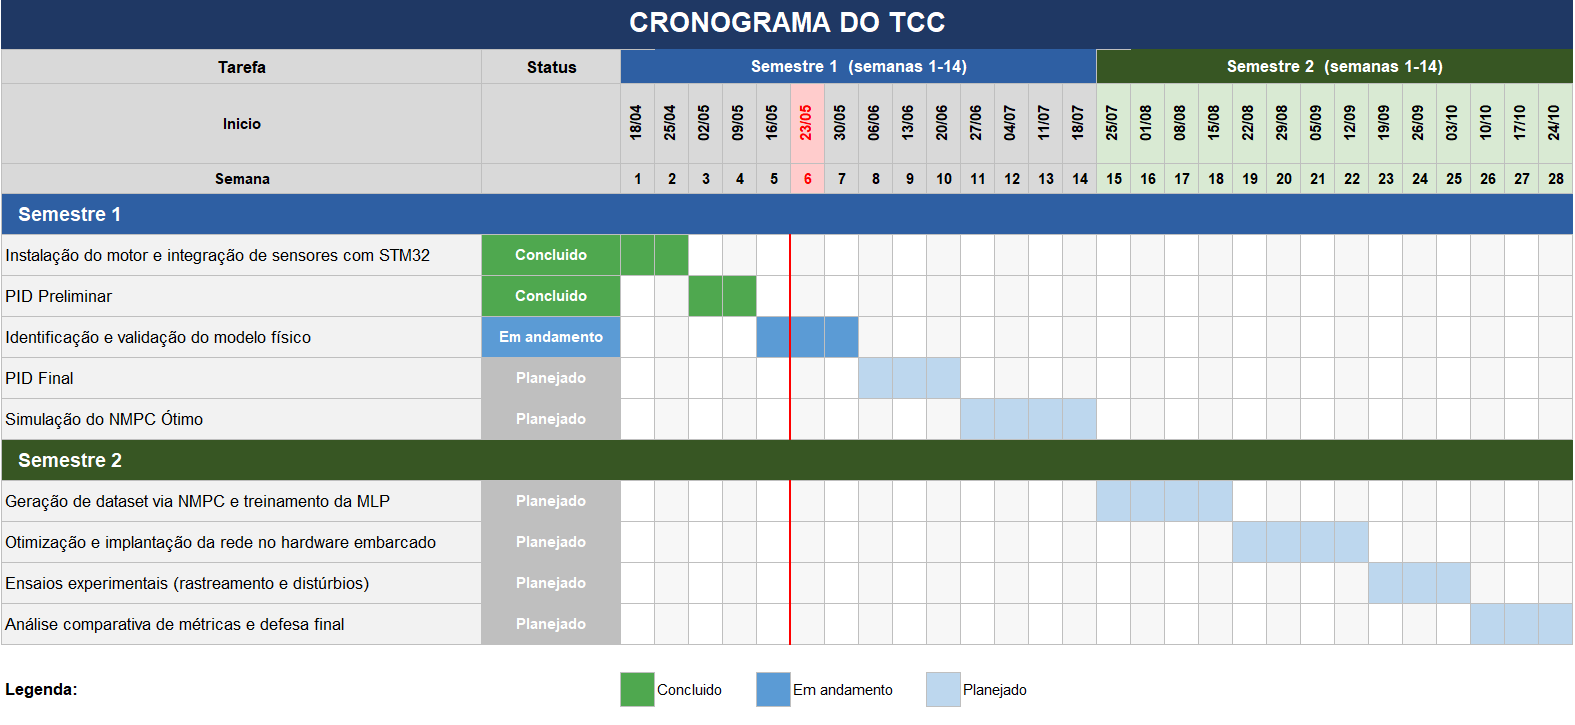
\includegraphics[width=1\textwidth]{img/cronograma-tcc.PNG}
    \caption{Cronograma do Projeto}
    \label{fig:cronograma-tcc}
\end{figure}


% ============================================================
\chapter{Procedimentos de Teste e Validação}

Os procedimentos de teste e validação estão organizados em quatro etapas  sequenciais, cobrindo desde a qualidade do modelo identificado até a  comparação final entre os três controladores implementados.

% ------------------------------------------------------------
\section{Validação do Modelo Identificado}

A qualidade do modelo grey-box obtido via \texttt{nlgreyest} será avaliada  sobre o conjunto de validação retido, composto pelos ensaios de degraus de  amplitude variada, conforme descrito na Seção~\ref{subsec:divisao_dados}.

Serão reportadas as seguintes métricas:

\begin{itemize}
    \item Coeficiente de ajuste (\textit{fit}\,\%) entre a trajetória angular simulada $\hat{\theta}(t)$ e a medida $\theta(t)$, com critério de aceite \textit{fit} $> 85\%$;
    \item Erro Quadrático Médio (RMSE) entre $\hat{\theta}(t)$ e $\theta(t)$;
    \item Análise de resíduos, verificando independência em relação à entrada, atestando a adequação estrutural do modelo;
    \item Resposta a degraus não utilizados na identificação, avaliando a capacidade de generalização do modelo.
\end{itemize}

% ------------------------------------------------------------
\section{Validação do Controlador PID}

O controlador PID será validado no sistema físico com os seguintes ensaios:

\begin{itemize}
    \item Rastreamento de referências em degrau nas amplitudes de 
          $30°$, $45°$ e $60°$, medindo tempo de acomodação e overshoot;
    \item Sequência de degraus com amplitudes variadas 
          ($60°$, $30°$, $-60°$, $-30°$), avaliando o comportamento 
          em toda a faixa de operação;
    \item Rejeição a distúrbio impulsivo aplicado manualmente ao braço do aeropêndulo durante operação em regime permanente;
    \item Registro do tempo de execução da rotina de controle no STM32, verificando o atendimento ao \textit{deadline} de $T_s = 10$\,ms.
\end{itemize}

% ------------------------------------------------------------
\section{Validação do NMPC Simulado}

O NMPC ótimo, desenvolvido offline via CasADi, será validado em simulação  antes da geração do dataset. Os critérios de avaliação são:

\begin{itemize}
    \item Comparação das trajetórias NMPC e PID sobre as mesmas referências de degrau, avaliando tempo de acomodação e overshoot;
    \item Verificação do respeito às restrições de entrada ($u \in [-0{,}3,\; 0{,}3]$) e de estado ao longo de toda a trajetória;
    \item Medição do tempo médio de resolução do NLP pelo solver CasADi, como referência de custo computacional do NMPC exato.
\end{itemize}

% ------------------------------------------------------------
\section{Validação da MLP Embarcada}

A rede neural implantada no STM32 via X-CUBE-AI será avaliada em duas etapas.

\subsection{Fidelidade à Política Ótima}

Sobre o conjunto de teste retido ($15\%$ do dataset), serão calculados:

\begin{itemize}
    \item Erro Quadrático Médio (MSE) e Erro Absoluto Médio (MAE) entre a ação de controle da MLP $\hat{u}$ e a do NMPC exato $u^*$;
    \item Distribuição dos erros de aproximação ao longo da faixa de estados de operação.
\end{itemize}

\subsection{Desempenho em Malha Fechada}

Os mesmos ensaios realizados para o PID (rastreamento, rejeição a  distúrbios e sequência de degraus) serão repetidos com a MLP, permitindo comparação direta. Adicionalmente, serão medidos:

\begin{itemize}
    \item Tempo de inferência da rede no STM32, que deve ser inferior a $T_s = 10$\,ms;
    \item Uso de memória Flash e SRAM após a implantação via X-CUBE-AI;
    \item Porcentagem de utilização de CPU durante a rotina de interrupção.
\end{itemize}

% ------------------------------------------------------------
\section{Análise Comparativa Final}

Os resultados dos três controladores serão consolidados na Tabela~\ref{tab:comparacao_controladores}, que constitui o principal resultado quantitativo do trabalho.

\begin{table}[h]
    \centering
    \caption{Comparação de desempenho entre os controladores avaliados.}
    \label{tab:comparacao_controladores}
    \begin{tabularx}{\textwidth}{Xccc}
        \hline
        \textbf{Métrica} & \textbf{PID} & \textbf{NMPC} & \textbf{MLP} \\
        \hline
        Tempo de acomodação médio (s)   & -- & -- & -- \\
        Overshoot máximo (\%)           & -- & -- & -- \\
        RMSE de rastreamento (graus)    & -- & -- & -- \\
        Tempo de execução por ciclo (ms)& -- & -- & -- \\
        Uso de CPU (\%)                 & -- & -- & -- \\
        Uso de Flash (KB)               & -- & -- & -- \\
        Uso de SRAM (KB)                & -- & -- & -- \\
        \hline
    \end{tabularx}
\end{table}